\documentclass[aspectratio=169]{beamer}

\usepackage[utf8]{inputenc}
\usepackage[english]{babel}
\usepackage{multicol}

\usepackage{mathtools}

\let\oldsection\section
\renewcommand{\section}[1]{
    \oldsection{#1}	
    \subsection{}
}

\setbeamerfont{section in toc}{size=\LARGE}

\newenvironment{myframe}[1][t]{\begin{frame}[#1]{\secname}{\subsecname}}{\end{frame}}

\usetheme{cranfielduniversity}

\usepackage[sorting=none, backend=biber, style=numeric, doi=false, isbn=false, url=false, eprint=false, date=year]{biblatex}

\addbibresource{../library.bib}
\addbibresource{../my_references.bib}

\author{Baptiste NOGARET}
\title{Food log analysis}

\supervisor{Dr Stefan RÜGER}

\setcounter{tocdepth}{1}

\begin{document}
	
	\begin{frame}[plain]
		\titlepage
	\end{frame}
    
    \begin{frame}{Table of contents}
        \begin{multicols}{2}
            \tableofcontents
        \end{multicols}
    \end{frame}
    
    \section{Why a food log analysis system?}
    
	\begin{myframe}
        Obesity / overweight in the world (lead to obesity, high blood pressure ... + cost)
        Best way to fight it: watch over what we eat
        With the progress of machine learning + access to more and more powerful device + widespread smartphone
        Proposition to automatize it
	\end{myframe}
    
    \section{Challenges}
    
    \begin{myframe}
        High intra-class variability
        Environment
        Way of taking the picture (zoom in or out)
        
        (Example)
    \end{myframe}
    
    \section{Overall process}
    
    \begin{myframe}
        Have a dataset of picture (from user ...)
        extract characteristic
        Segmentate
        Classify (learn)
        Estimate calory / quality intake
        Focus on the first three parts
    \end{myframe}
    
    \section{Dataset}
    
     \begin{myframe}
         \begin{center}
             \setlength{\tabcolsep}{5pt} % Default value: 6pt
             \renewcommand{\arraystretch}{1.5} % Default value: 1
             \begin{tabular}{||c | c c c c c||} 
                 \hline
                 Name & Size & Type of food & Number of classes & multiple food items per image & best known accuracy \\
                 \hline\hline
                 PFID & 6 & 6  & 87837 & 787 & 7 \\ 
                 \hline
                 UEC FOOD 256 & 6 & 6  & 87837 & 787 & 7 \\ 
                 \hline
                 UEC FOOD 100 & 6 & 6  & 87837 & 787 & 7 \\ 
                 \hline
             \end{tabular}
        \end{center}
         
         (Available dataset
         PFID
         FooDD
         
         UECFOOD 100 and 256)
         
         Criteria: 
         
         Highligth UEC FOOD 256
         
         Choose UECFOOD 256: segmentation, 256 classes (challenging)
         Different international categories ex: Japanese (rice, )
    \end{myframe}
    
    \subsection{Example of multi-items}
    
    \begin{myframe}
        \begin{figure}[h]
            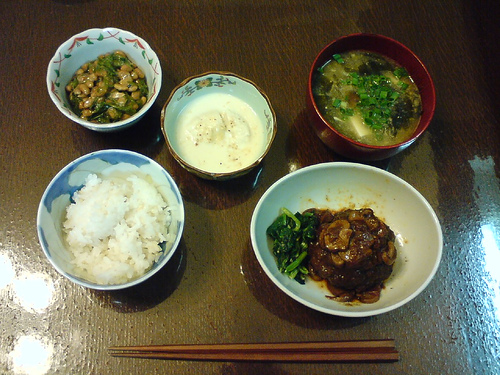
\includegraphics[width=0.4\textwidth,  height=0.4\textwidth ]{../img/multiple_food_items_1}
            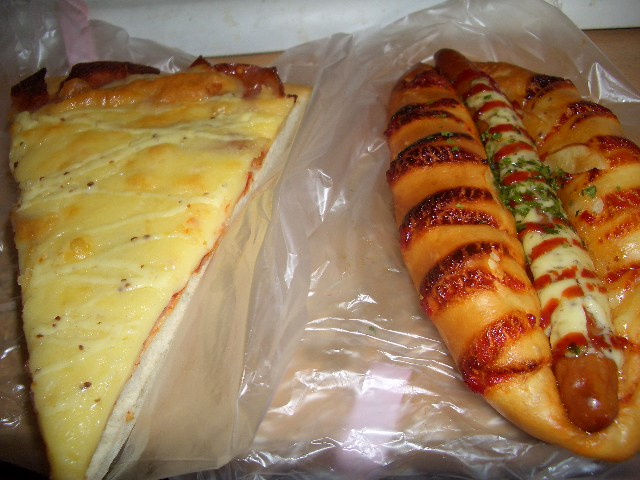
\includegraphics[width=0.4\textwidth,  height=0.4\textwidth ]{../img/multiple_food_items_4}
        \end{figure}
    \end{myframe}
    
    \section{Feature description}
    
    \subsection{Bag of visual words}
    
    \begin{myframe}
        Overall process:
        \begin{enumerate}
            \item Keypoints detection (dense grid / SIFT \footfullcite{Lowe2004} / SURF)
            \item Keypoints description (SIFT or SURF)
            \item Clustering to get N words (k-means clustering)
            \item Express each picture by an histogram of visual words
        \end{enumerate}
    \end{myframe}
    
    \subsection{Local binary pattern}
    
    \begin{myframe}
        content...
    \end{myframe}
    
    \subsection{Color moments and histograms}
    
    \begin{myframe}
        Mean, variance
        Hu moment?
        
        Color histogram (joint histogram)
        HSV channel
    \end{myframe}
    
    \section{Classifiers}
    
    \subsection{Tree and random forest}
    
    \begin{myframe}
        a decision tree recursively partitions the space such that the samples with the same labels are grouped together
        
        each recursion, it separates the data in a left and right partition for a feature j and a threshold
        
        threshold value is selected as the one that minimize the impurity (using impurity function such as Gini)
        
        Continue to split until the impurity can't be reduced or some pre-set stopping rules are met. Alternatively, the data are split as much as possible and then the tree is later pruned.
        
        Random forest: randomized decision tree. . The prediction of the ensemble is given as the averaged prediction of the individual classifiers.
    \end{myframe}
    
    \subsection{SVM}
    
    \begin{myframe}
        A Support Vector Machine (SVM) : try to find the set of hyperplanes to separate the different classes
        a good separation is achieved by the hyper-plane that has the largest distance to the nearest training data points of any class (so-called functional margin), since in general the larger the margin the lower the generalization error of the classifier.
        Use for classification or regression
        Linear model: it suppose a hyperplane separate the data
        
        Kernel trick: Idea : transform the initial space $\mathbb{R}^N$ to a higher dimensional space $\mathbb{R}^M$ (where $M > N$) where a hyperplane can sepearet this data
        
        Example of kernel: kernel function: 
        $\chi^2$ kernel: $k(x,y) = 1 - \displaystyle\sum_{i=1}^n \frac{(x_i-y_i)^2}{\frac{1}{2}(x_i+y_i)}$
        
    \end{myframe}
    
    \subsection{CNN}
    
    \begin{myframe}
        Convolutional Neural Networks are very similar to ordinary Neural Networks from the previous chapter: they are made up of neurons that have learnable weights and biases. Each neuron receives some inputs, performs a dot product and optionally follows it with a non-linearity. The whole network still expresses a single differentiable score function: from the raw image pixels on one end to class scores at the other. And they still have a loss function (e.g. SVM/Softmax) on the last (fully-connected) layer and all the tips/tricks we developed for learning regular Neural Networks still apply.
        
        mainly use when the input is an image: neurons arranged in 3 dimensions: width, height, depth
        
        Main layer:
        Convolutional layer
        Pooling layer
        Activation layer: mainly relu (rectified linear unit): max(0, x)
        Fully-connected layer
    \end{myframe}
    
    \section{Segmentation}
    
    \begin{myframe}
        CNN pre-trained for saliency detection (PASCAL VOC / 19 layers)
    \end{myframe}
    
    \section{Results}
    
    \subsection{Segmentation}
    
    \begin{myframe}
        Precision, recall, accuracy (+ their definition)
        
        Result for UECFOOD 256
        
        (Display graph of the accuracy / recall / precision function of the overlaping value)
    \end{myframe}
    
    \subsection{Classification}
    
    \begin{myframe}
        Results for :
        - CNN as feature descriptors
        - Color histogram
        - BoW
        
        Compare to other results
    \end{myframe}
    
    \subsection{Segmentation followed by classification}
    
    \begin{myframe}
        Combining segmentation and classification:
        
        Overall accuracy: 28 \%
        74 \% for segmentation
        38 \% for classification

        Compare to other results
        
        (Show the 5 best / least classes' accuracy)
        (Show the most confusing items)
    \end{myframe}
    
    \section{Future work}
    
    \begin{myframe}
        Regroup the classification in 5 big categories
    \end{myframe}
    
    \begin{frame}{Food log analysis - Baptiste NOGARET}        
        \begin{columns}
            
            \column{0.5\textwidth}
            Segmentation and classfication applied on two reference datasets
            
            Obtain better segmentation than the reference
            
            Overall accuracy of 28 \% (to date, best result is 36 \% in ...).
            
            \column{0.5\textwidth}
            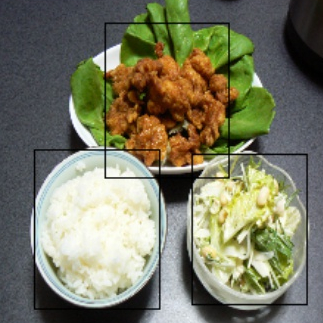
\includegraphics[width=\textwidth]{../img/seg_97_gt}
        \end{columns}
    \end{frame}
   
\end{document}